
\documentclass[11pt,a4paper,openany,oneside]{abntex2}
%\usepackage[latin1]{inputenc}
\usepackage[utf8]{inputenc}
\usepackage[brazil]{babel}
\usepackage[T1]{fontenc}
\usepackage{amsmath}
\usepackage{makeidx}
\usepackage{lipsum}
\usepackage{graphicx}
\usepackage{cite} 
\usepackage{indentfirst}
\usepackage{listings}
\usepackage{float}
\usepackage{multirow}
\usepackage{pdflscape}
\usepackage{scalefnt}
\usepackage{subfigure}

\lstset{
	basicstyle = {\footnotesize},
	numbers=left,
	firstline=1,
	language=Java,
	%frame=leftline|topline,
	frame=single,
	tabsize=2,
	breaklines=true
}



%\lstset{
%language = C++, % Linguagem de programação
%basicstyle = \footnotesize, % Tamanho da fonte do código
%numbers = left, % Posição da numeração das linhas
%numberstyle = \tiny\color{blue}, % Estilo da numeração de linhas
%stepnumber = 1, % Numeração das linhas ocorre a cada quantas linhas?
%numbersep = 10pt, % Distância entre a numeração das linhas e o código
%backgroundcolor = \color{white}, % Cor de fundo
%showspaces = false, % Exibe espaços com um sublinhado
%showstringspaces = false, % Sublinha espaços em Strings
%showtabs = false, % Exibe tabulação com um sublinhado
%frame = trBL, % Envolve o código com uma moldura, pode ser single ou trBL
%rulecolor = \color{black}, % Cor da moldura
%tabsize = 2, % Configura tabulação em x espaços
%captionpos = b, % Posição do título pode ser t (top) ou b (bottom)
%breaklines = true, % Configura quebra de linha automática
%breakatwhitespace= false, % Configura quebra de linha
%title = \lstname, % Exibe o nome do arquivo incluido
%caption = \lstname, % Também é possível usar caption no lugar de title
%keywordstyle = \color{blue}, % Estilo das palavras chaves
%commentstyle = \color{dkgreen}, % Estilo dos Comentários
%stringstyle = \color{mauve}, % Estilo de Strings
%escapeinside = {\%*}{*)}, % Permite adicionar comandos LaTeX dentro do seu código
%morekeywords     ={*,...} % Se quiser adicionar mais palavras-chave
%}%

\begin{document}
	\begin{titlepage}
		\vfill
		\begin{center}
			{\large \textbf{Universidade Federal de Ouro Preto}} \\[2.5cm]
			
			  
			{\large \textbf{Mateus Oliveira dos Santos - 11.2.8093}}\\[4cm]
			
			
			{\Large Exercício Extra}\\[4cm]
			
			\hspace{.45\textwidth} %posiciona a minipage
			\begin{minipage}{.5\textwidth}
				\large Trabalho Extra apresentado a disciplina de Avaliação e Desempenho de Sistemas Computacionais do curso de Engenharia de Computação do  Instituto de Ciências Exatas e Aplicadas da  Universidade  Federal de Ouro Preto.\\[1cm]
				Professor Alexandre Magno de Sousa.
			\end{minipage}
			\vfill
			
			\vspace{2cm}
			
			\large \textbf{João Monlevade - MG}
			
			\large \textbf{Fevereiro 2016}
		\end{center}
	\end{titlepage}	
	
	
	
\chapter{Enunciado}
\label{enunciado}
%\section{\textbf{Enunciado}}
	
	1. Um servidor de banco de dados possui uma CPU e dois discos, o monitor de desempenho do SGBD, que realiza medições em nível de transações, gerou um log de atividades dos recursos do sistema para cada transação que ocorreram em um intervalo de 2 minutos e meio. Ao todo 200 transações foram registradas nesse período de tempo conforme os dados da planilha anexa “DBMS-Performance-Monitor-Log.xls” (tempo de CPU e número de I/Os para cada disco, além do ID para cada transação). Para realizar a caracterização do workload do servidor, faça o que se pede:
	
	(a) apresente uma tabela com informações com estatísticas básicas para cada feature registrada, tais como: média, variância, desvio padrão, coeficiente de variação, valor total (soma), valores mínimo e máximo, range (faixa de valores abrangido, e.g. máximo - mínimo), 1o quartil, 2o quartil e 3o quartil.
	
	(b) apresente gráficos para cada feature tais como: histograma de único parâmetro, \textit{Cumulative Distribution Function} (CDF) e Box Plot.
	
	(c) realize a Análise do Componente Principal (PCA) seguindo todos os passos apresentados em sala de aula, não se esqueça de construir os gráficos.
	
	(d) construa uma tabela de correlação conforme a Tabela 1, em que $R_{(i,j)}$ representa a correlação da feature i com o principal fator \textit{j} calculado pelo PCA de acordo com a equação
	\begin{equation}
	R_{(i,j)} = \frac{\frac{1}{n-1} \sum_{k}^{n}(i_k-\hat{i})(j_k-\hat{j})}{S_i  S_j}
	\end{equation}
	
	
	
	
	onde \textit{n} representa o número total de componentes registrados, $\hat{i}$ e $\hat{j}$ são médias, $S_i$ e
	$S_j$ são o desvio padrão, e $i_k$ e $j_k$ representam os dados de cada componente da \textit{feature i} e do principal fator \textit{j}.
	
	A partir dessa tabela, elabore um gráfico do tipo plano cartesiano onde cada \textit{feature} (Tempo de CPU, \# de I/Os do disco 1 e 2) sejam representados como pontos $(x, y)$ onde $x$ é o valor de correlação com o Principal Fator 1 e $y$ é o valor de correlação com o Principal Fator 2. Esse gráfico mostrará a relação dos dados medidos com os principais fatores, geralmente é mais utilizado para dados com alta dimensionalidade, $n > 3$, isto é, quanto maior os valores de correlação com os principais fatores $y_1$ e $y_2$, maior é a influência desses fatores na componente de dados.
	
	(e) mostre os resultados, faça observações e apresente conclusões
	
	\begin{table}[htbp]
		\centering
		\caption{Tabela de análise PCA} 
		
		\begin{tabular}{lcc}
			\toprule
		 Programa    & Principal Fator 1 ($y_1$) &Principal Fator 2 ($y_2$)\\
			\midrule
		Tempo de CPU     & $R_{(cpu,y1)}$        & $R_{(cpu,y_2)}$   \\
		\# I/Os Disco 1  & $R_{(I/OsDisco1,y_1)}$ & $R_{(I/OsDisco1,y_2)}$    \\
		\# I/Os Disco 2  & $R_{(I/OsDisco2,y_1)}$ & $R_{(I/OsDisco2,y_2)}$       \\
		%\multicolumn{7}{l}{\textit{caption fonte wwww}} \\
			\bottomrule
		\end{tabular}%
		%\namedlegend{teste legend}
		\label{tab:apca}%
	\end{table}%

\textbf{Observação:} para criação dos gráficos CDF e Box Plot, que não foram apresentados na disciplina, realize uma pesquisa em estatística para ter conhecimento de como se constrói esse tipo de gráfico.

\chapter{Introdução}	

O trabalho apresenta a resolução do problema proposto na seção de enunciado \ref{enunciado}. A seção \ref{qe} apresenta as observações e conclusões obtidas a partir da análise dos dados resultantes das seções de \ref{qa} a  \ref{qd}. As seções seguem a ordem da resolução do problema proposto, exceto pela questão \textbf{e} que será a primeira a ser apresentada.
	
\chapter{Análise dos resultados - Questão E}
\label{qe}
Apresentaremos as conclusões e observações de acordo com a sequencia de resolução das questões.
\section{Questão A}
\label{qea}
As tabelas \ref{tab:dadosestat} e \ref{tab:dados} apresentam os dados estatísticos do problema e os dados reais parciais, para acesso aos dados completos acesse o repositório do git citado em \ref{qas}. Como esperado os dados normalizados possuem média zero e desvio padrão um. Além dos somatórios igual a zero das componentes normalizadas e dos fatores do PCA. As observações dos gráficos explicaram melhor o que cada resultado significa na seção \ref{qeb}.

\section{Questão B}
\label{qeb}

Analisando os histogramas na seção \ref{qbh} podemos observar que as concentrações de cargas que tomam maior de tempo de cpu se encontram entre 75 ms e 172ms, e uma segunda carga aparentemente média entre 412 ms e 508ms.
Para o disco 1 a maioria das transações, cerca de 50,  executam aproximadamente 16 IOs enquanto que para o disco 2 são 30 IOs por transação, com uma frequência igual ao disco 1. No disco um as demais transações estão mais distribuídas, enquanto que no disco 2 as transações com maior quantidade de IOs estão entre 64 e 80 IOs por transação.

Ao se observar os gráficos das CDFs \ref{qbcdf} podemos  fornecer um dado mais preciso, onde cerca de $60\%$ das operações na CPU  gastam aproximadamente 400ms de tempo de CPU.
No disco 1 apenas $30\%$ das transações fazem até 30 IOs , já no disco 2 aproximadamente $26\%$ das transações fazem até 40 IOs.

 Com o box plot conseguimos entender melhor as curvas das CDFs dos disco, como podemos ver no gráfico da figura \ref{fig:boxplotd1d2} enquanto do disco 1 apresenta maior variabilidade entre o primeiro quartil e a mediana, o disco 2 é o oposto. Apesar dos máximos e mínimos estarem próximos os tipo de carga que cada disco recebe varia claramente em número de IOs, ou seja, o disco dois recebem operações que fazem mais IOs que o disco 1.
 
 O box plot do CPU \ref{fig:boxplotcpu} mostra que a maior parte das operações tem variabilidade em tempo de CPU entre a mediana e o terceiro quartil.



\section{Questão C}
\label{qec}

Realizando o PCA encontramos que o principal fator 1 é o disco 1, com cercar de $58\%$ de representação dos dados e o principal fator 2 é a CPU, com cercar de $35\%$ de representação dos dados. Logo, o disco 2 com aproximadamente $7\%$.

Observando o gráfico \ref{fig:pca} podemos observar que, apesar de uma dispersão próximo ao valor dois do principal fator 2 (CPU), a maior parte dos dados se concentram ao longo do eixo do principal fator 1 (Disco 1 ). De certa forma, era de se esperar que o principal fator 1 tinha grande chances de ser um dos disco por se tratar de um sistema de banco de dados.


\section{Questão D}
\label{qed}

Por fim, observando o gráfico \ref{fig:pcacomp} onde o eixo x é o principal fator 1 e o eixo y é o principal fator 2, podemos observar que o disco 1 realmente se aproxima do eixo do principal fator 1 e a CPU idem ao eixo y. O disco 2, como analisado no PCA representa pouco os dados, e o gráfico \ref{fig:pcacomp} evidencia esse fato, o ponto disco 2 está disperso do eixo x e do eixo y, confirmando os resultados obtido pelo PCA.


\chapter{Dados -Questão A}
\label{qa}


\section{\textbf{Software Utilizados}}
\label{qas}
	Para o desenvolvimento do trabalho utilizamos o software editor de planilhas OpenOffice Calc e o Calcular autovalores e autovetores de uma matriz do Wolfram Alpha\cite{img}.
	Todos os dados estão disponíveis no repositório \textit{https://github.com/mateusstp/avaliacaodesempenhosistemas}.



\section{\textbf{Dados do problema e dados estatísticos }}
\label{qade}
%\begin{landscape}
	
	\begin{table}[H]
		\caption{Dados do problema e dados estatísticos}
		\scalefont{0.6}
		\centering
		\begin{tabular}{|c|c|c|c|c|c|c|c|c|c|c|}
			\hline
			\textbf{} & \multicolumn{ 3}{c|}{\textbf{Coleta Real}} & \textbf{} & \multicolumn{ 3}{c|}{\textbf{Normalizado}} & \multicolumn{ 3}{c|}{\textbf{Saídas}} \\ \hline
			\textbf{Número} & \textbf{CPU} & \textbf{Disk 1} & \textbf{Disk 2} & \textbf{TR ID } & \textbf{CPU} & \textbf{Disk 1} & \textbf{Disk 2} & \textbf{y1} & \textbf{y2} & \textbf{y3} \\ \hline
			1 & 116,824 & 9,000 & 9,000 & 18 & -0,732 & -1,570 & -1,357 & 0,544 & 1,942 & -0,879 \\ \hline
			2 & 64,383 & 7,000 & 9,000 & 37 & -1,048 & -1,644 & -1,357 & 0,696 & 2,162 & -0,695 \\ \hline
			3 & 35,403 & 7,000 & 9,000 & 58 & -1,223 & -1,644 & -1,357 & 0,801 & 2,248 & -0,585 \\ \hline
			4 & 104,409 & 8,000 & 12,000 & 77 & -0,807 & -1,607 & -1,243 & 0,498 & 1,990 & -0,755 \\ \hline
			5 & 119,793 & 9,000 & 8,000 & 19 & -0,714 & -1,570 & -1,395 & 0,557 & 1,940 & -0,919 \\ \hline
			. & . & . & . & . & . & . & . & . & . & . \\ \hline
			. & . & . & . & . & . & . & . & . & . & . \\ \hline
			. & . & . & . & . & . & . & . & . & . & . \\ \hline
			198 & 139,368 & 60,000 & 40,000 & 57 & -0,596 & 0,320 & -0,183 & 0,628 & 0,057 & 0,306 \\ \hline
			199 & 136,998 & 68,000 & 37,000 & 201 & -0,610 & 0,616 & -0,297 & 0,852 & -0,167 & 0,292 \\ \hline
			200 & 149,211 & 69,000 & 38,000 & 17 & -0,537 & 0,653 & -0,259 & 0,802 & -0,242 & 0,282 \\ \hline
			$\sum x$ & 47640,823 & 10275,000 & 8969,000 & - & 0,000 &0,000& 0,000 & 0,000 & 0,000 & 0,000 \\ \hline
			$\sum x^{2}$    & 16822813,796 & 672893,000 & 541135,000 & - & 199,000 & 199,000 & 199,000 & 207,390 & 348,108 & 41,503 \\ \hline
			Média & 238,204 & 51,375 & 44,845 & - & 0,000 & 0,000 & 0,000 & 0,000 & 0,000 & 0,000 \\ \hline
			Variância & 27510,420 & 728,718 & 698,091 & - & 1,000 & 1,000 & 1,000 & 1,042 & 1,749 & 0,209 \\ \hline
			Desvio Padrão & 165,863 & 26,995 & 26,421 & - & 1,000 & 1,000 & 1,000 & 1,021 & 1,323 & 0,457 \\ \hline
		\end{tabular}
		\label{tab:dados}
	\end{table}
%\end{landscape}

\begin{table}[htbp]
	\caption{Dados  estatísticos}
	\centering
	\begin{tabular}{|c|c|c|c|}
		\hline
		& \textbf{CPU} & \textbf{Disk 1} & \textbf{Disk 2} \\ \hline
		\hline
		\textbf{Coeficiente de Variação} & 0,696 & 0,525 & 0,589 \\ \hline
		\textbf{Valor Máximo} & 507,450 & 85,000 & 92,000 \\ \hline
		\textbf{Valor Mínimo} & 23,597 & 5,000 & 7,000 \\ \hline
		\textbf{Range} & 483,853 & 80,000 & 85,000 \\ \hline
		\textbf{1º Quartil} & 104,439 & 33,000 & 26,250 \\ \hline
		\textbf{2º Quartil} & 151,625 & 63,000 & 39,000 \\ \hline
		\textbf{3º Quartil} & 418,052 & 72,000 & 68,000 \\ \hline
		\textbf{Mediana} & 151,625 & 63,000 & 39,000 \\ \hline
	\end{tabular}
	\label{tab:dadosestat}
\end{table}


\chapter{Gráficos - Questão B}
%\section{\textbf{Gráficos  - Questão b}}
\label{qb}
\section{\textbf{Histogramas}}
\label{qbh}
\begin{figure}[H]
	\begin{minipage}[b]{0.45\linewidth}
		\centering
		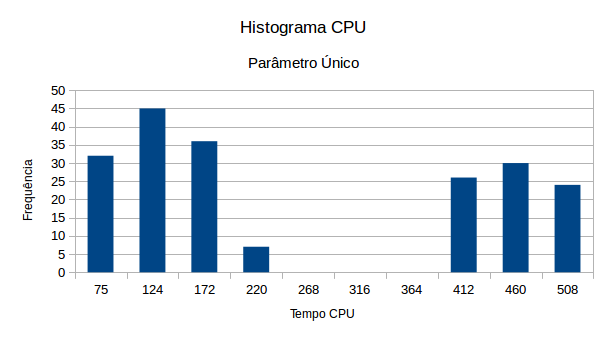
\includegraphics[width=\textwidth]{histogramacpu.png}
		\caption{Histograma CPU com 10 Classes}
		\label{fig:histocpu}
	\end{minipage}
	\hspace{0.5cm}
	\begin{minipage}[b]{0.45\linewidth}
		\centering
		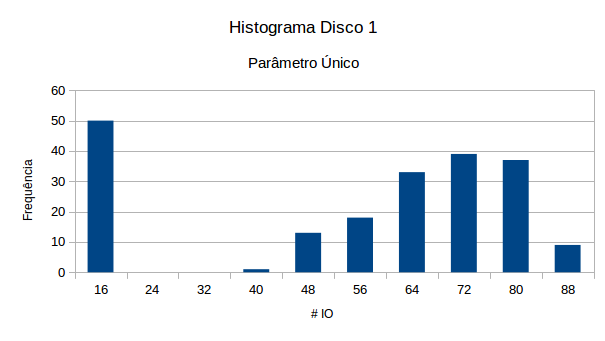
\includegraphics[width=\textwidth]{histogranadsico.png}
		\caption{Histograma Disco 1 com 10 Classes}
		\label{fig:histod1}
	\end{minipage}
	\hspace{0.5cm}
	\begin{minipage}[t]{0.45\linewidth}
		\centering
		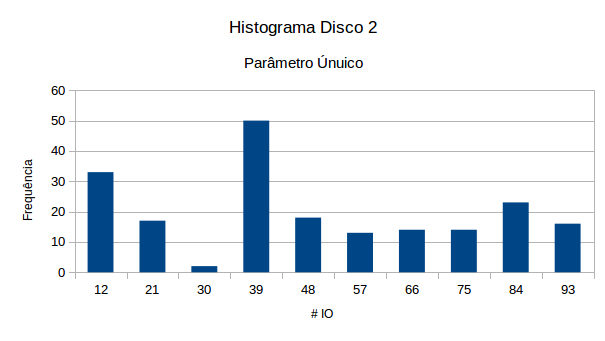
\includegraphics[width=\textwidth]{histogramadsic2.png}
		\caption{Histograma Disco 2 com 10 Classes}
		\label{fig:histod2}
	\end{minipage}
		
\end{figure}


%	\begin{figure}[H]
%			\centering%
%			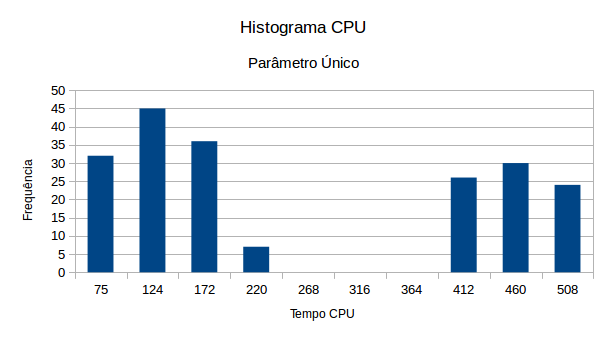
\includegraphics[scale=0.80]{histogramacpu.png}
%			\caption{Histograma CPU com 10 Classes}
%		\label{fig:histocpu}
%		\end{figure}

%	\begin{figure}[H]
%		\centering%
%		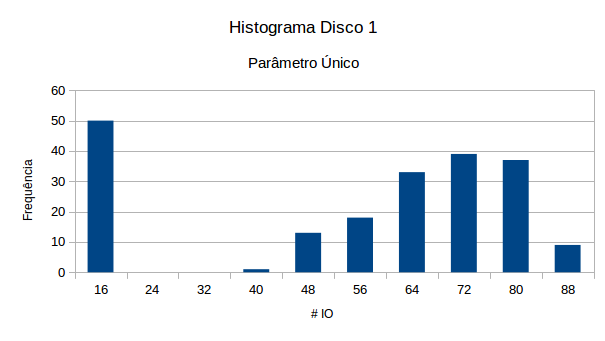
\includegraphics[scale=0.80]{histogranadsico.png}
%		\caption{Histograma Disco 1 com 10 Classes}
%		\label{fig:histod1}
%	\end{figure}

%	\begin{figure}[H]
%		\centering%
%		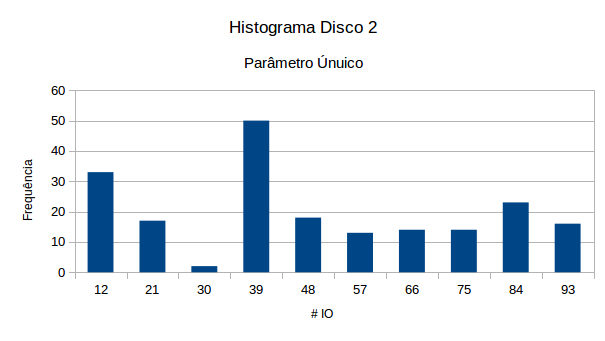
\includegraphics[scale=0.80]{histogramadsic2.png}
%		\caption{Histograma Disco 2 com 10 Classes}
%		\label{fig:histod2}
%	\end{figure}
	
\section{\textbf{CDF }}
\label{qbcdf}
\begin{figure}[H]
	\begin{minipage}[b]{0.45\linewidth}
		\centering
		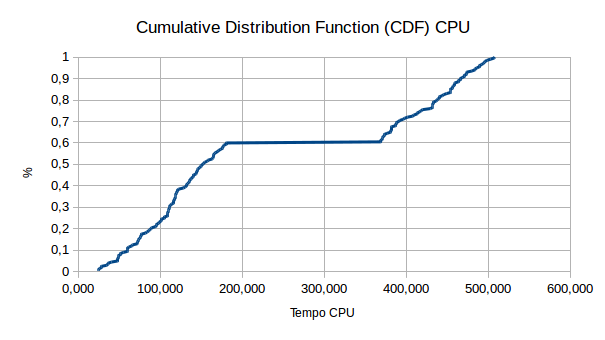
\includegraphics[width=\textwidth]{cdfcpu.png}
		\caption{CDF CPU}
		\label{fig:cfdcpu}
	\end{minipage}
    \hspace{0.5cm}
	\begin{minipage}[b]{0.45\linewidth}
		\centering
		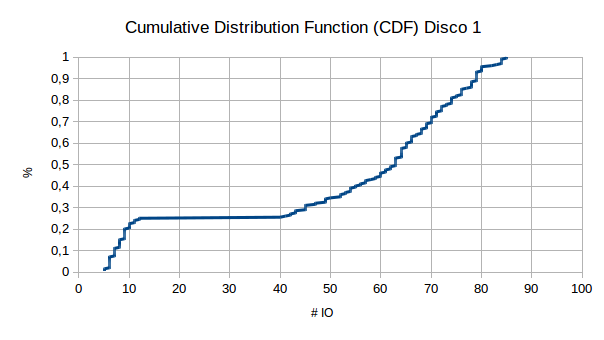
\includegraphics[width=\textwidth]{cdfdisco1.png}
		\caption{CDF Disco 1}
		\label{fig:cfdd1}
	\end{minipage}
	\hspace{0.5cm}
	\begin{minipage}[t]{0.45\linewidth}
		\centering
		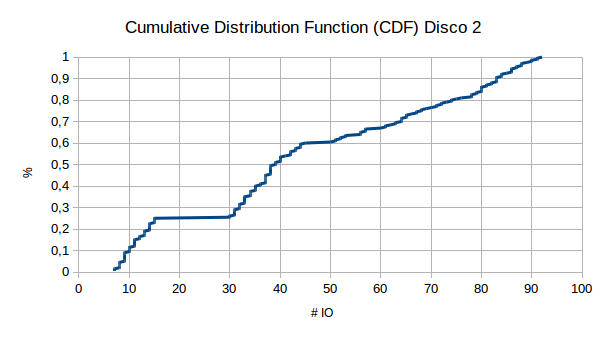
\includegraphics[width=\textwidth]{cdfdisco2.png}
		\caption{CDF Disco 2}
		\label{fig:cfdd2}
	\end{minipage}
	
\end{figure}


%	\begin{figure}[H]
%		\centering%
%		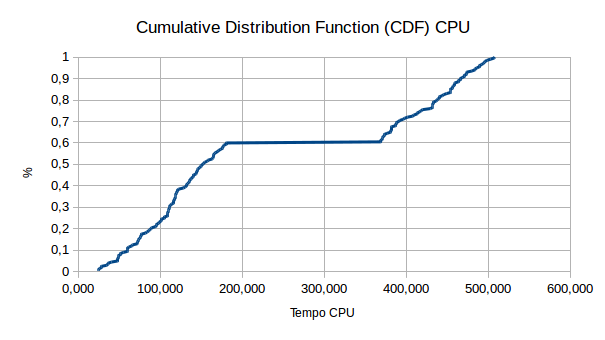
\includegraphics[scale=0.80]{cdfcpu.png}
%		\caption{CDF CPU}
%		\label{fig:cfdcpu}
%	\end{figure}

%	\begin{figure}[H]
%		\centering%
%		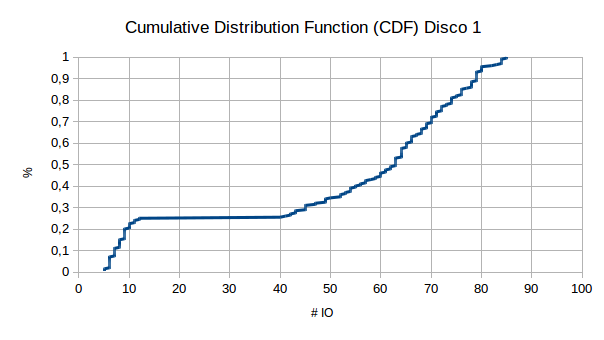
\includegraphics[scale=0.80]{cdfdisco1.png}
%		\label{fig:cfdd1}
%	\end{figure}

%	\begin{figure}[H]
%		\centering%
%		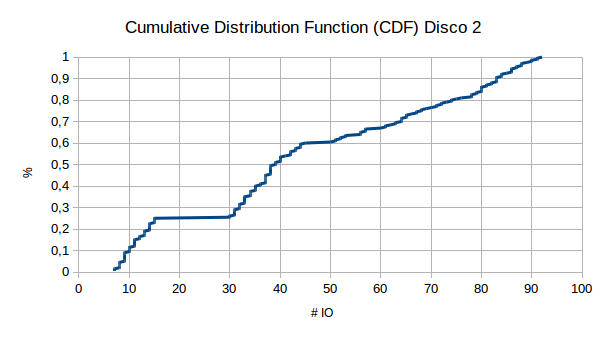
\includegraphics[scale=0.80]{cdfdisco2.png}
%		\caption{CDF Disco 2}
%		\label{fig:cfdd2}
%	\end{figure}
	
\section{\textbf{Box Plot}}
\label{qbboxp}
\begin{figure}[H]
	\begin{minipage}[b]{0.45\linewidth}
		\centering
		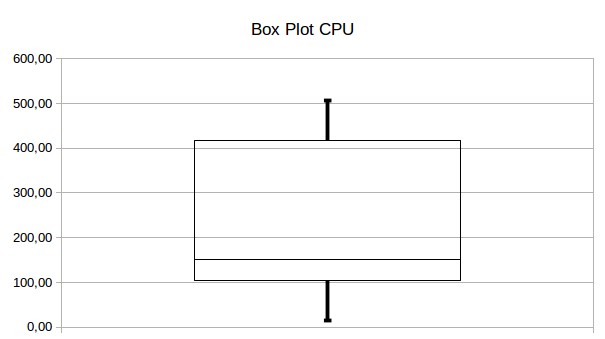
\includegraphics[width=\textwidth]{boxplotcpu.png}
		\caption{Box plot CPU}
		\label{fig:boxplotcpu}
	\end{minipage}
	\hspace{0.5cm}
	\begin{minipage}[b]{0.45\linewidth}
		\centering
		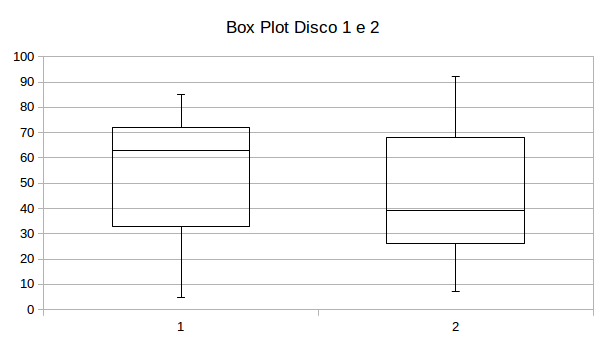
\includegraphics[width=\textwidth]{boxplotdiscos.png}
		\caption{Box plot Disco 1 e 2}
		\label{fig:boxplotd1d2}
					
	\end{minipage}
	
\end{figure}
	
%	\begin{figure}[H]
%		\centering%
%		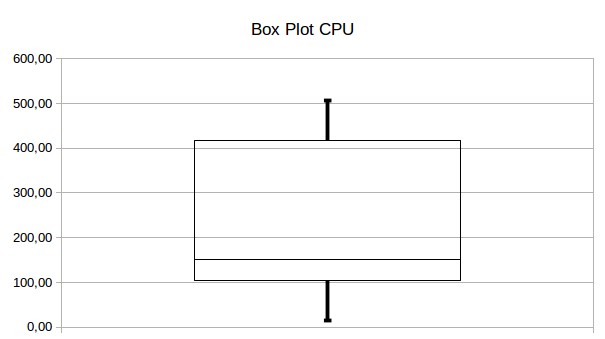
\includegraphics[scale=0.80]{boxplotcpu.png}
%		\caption{Box plot CPU}
%		\label{fig:boxplotcpu}
%	\end{figure}
	
%		\begin{figure}[H]
%			\centering%
%			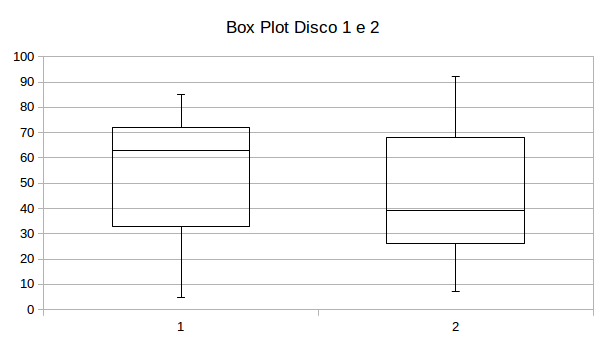
\includegraphics[scale=0.80]{boxplotdiscos.png}
%			\caption{Box plot Disco 1 e 2}
%			\label{fig:boxplotd1d2}
%		\end{figure}				
%




\chapter{Análise do Componente Principal - Questão C}
\label{qc}
%\section*{\textbf{Análise do Componente Principal - Questão c}}

\begin{table}[H]
		\begin{minipage}[b]{0.45\linewidth}
			\centering
			\caption{Autovetores}
			\begin{tabular}{|c|c|c|}
				\toprule
				\textbf{v1} &  \textbf{v2} &  \textbf{v3}  \\ \hline
				-0,596 & 0,485 & -0,640 \\ \hline
				-0,496 & -0,849 & -0,181 \\ \hline
				-0,631 & 0,209  & 0,747 \\ 
				\bottomrule
			\end{tabular}
			\label{tab:autovetores}	
		\end{minipage}
		\hspace{0.5cm}
		\begin{minipage}[b]{0.45\linewidth}
			\centering
			\caption{Matriz de Correlação} 
			\begin{tabular}{|l|c|c|c|}
				\toprule
				1,00 & 0,465 & 0,916\\ \hline
				0,465 & 1,00 & 0,626\\ \hline
				0,916 & 0,626	& 1,00\\ 
				
				\bottomrule
			\end{tabular}%
			%\namedlegend{teste legend}
			\label{tab:matrizcorrelacao}%
			
		\end{minipage}
\end{table}%




\begin{table}[H]
	\centering
	\caption{Correlação entre variáveis} 
	\begin{tabular}{lccc}
		\toprule
		    Correlação & $(CPU,Disco 1)$ & $(CPU,Disco 2)$ & $(Disco 1,Disco 2)$\\
		\midrule
		$R_{(i,j)}$    & 0,465  & 0,916	& 0,626\\
		\bottomrule
	\end{tabular}%
	%\namedlegend{teste legend}
	\label{tab:correlacao}%
\end{table}%

%\begin{table}[H]
%	\centering
%	\caption{Matriz de Correlação} 
%	\begin{tabular}{|l|c|c|c|}
%		\toprule
%		1,00 & 0,465 & 0,916\\ \hline
%		0,465 & 1,00 & 0,626\\ \hline
%		0,916 & 0,626	& 1,00\\ 
		
%		\bottomrule
%	\end{tabular}%
	%\namedlegend{teste legend}
%	\label{tab:correlacao}%
%\end{table}%



%		&\multicolumn{ 3}{c|}{\textbf{Autovetores}}  & \\ \hline
%\begin{table}[H]
%	\caption{Autovetores}
%		\centering
%	\begin{tabular}{|c|c|c|}
%				\toprule
%		\textbf{v1} &  \textbf{v2} &  \textbf{v3}  \\ \hline
%		-0,596 & 0,485 & -0,640 \\ \hline
%		-0,496 & -0,849 & -0,181 \\ \hline
%		-0,631 & 0,209  & 0,747 \\ 
%		\bottomrule
%	\end{tabular}
%	\label{autovetores}
%\end{table}


\begin{table}[h]
	\caption{Porcentegem PCA}
		\centering
	\begin{tabular}{|c|c|c|c|}
		\hline
		& \textbf{CPU} & \textbf{Disk 1} & \textbf{Disk 2} \\ \hline
		\hline
		\textbf{Porcentagem de cada fator} & 34,74\% & 58,31\% & 6,95\% \\ \hline
	\end{tabular}
	\label{tab:porcentagenpca}
\end{table}


	\begin{figure}[H]
		\centering%
		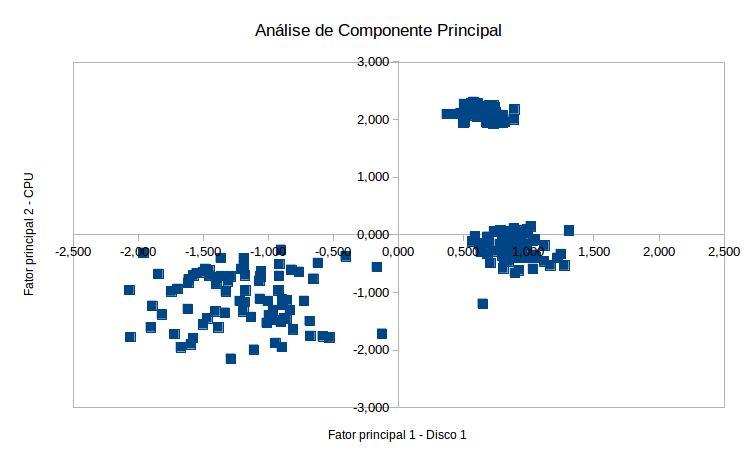
\includegraphics[scale=0.60]{pca.png}
		\caption{PCA }
		\label{fig:pca}
	\end{figure}


\chapter{Correlação PCAs e Componentes - Questão D}
\label{qd}

\begin{table}[H]
	\caption{Correlação PCA e Componentes}
	\centering
	\begin{tabular}{|l|c|c|}
		\hline
		\textbf{}     & \textbf{y1} & \textbf{y2} \\ \hline
		$R_{(pcu,yi)}$ & -0,799       & -0,938 \\ \hline
		$R_{(d1,yi)}$  & -0,902       & -0,189 \\ \hline
		$R_{(d2,yi)}$  & -0,882       & -0,865 \\ \hline
	\end{tabular}
	\label{tab:pcaconponentes}
\end{table}

	\begin{figure}[H]
		\centering%
		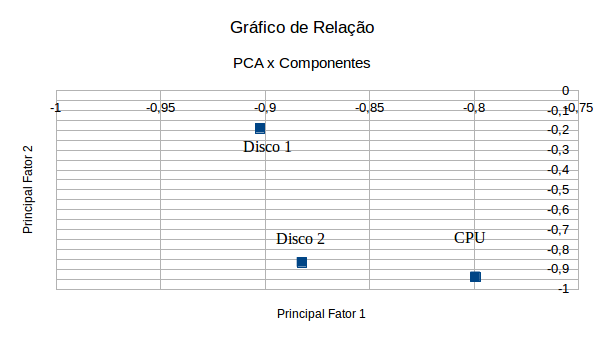
\includegraphics[scale=0.80]{relacao.png}
		\caption{Correlação PCA e Componentes}
		\label{fig:pcacomp}
	\end{figure}





	%\begin{figure}[H]
%		\centering%
%		\includegraphics[scale=0.50]{geral.png}
%		\caption{Diagrama Projeto TP1}
%		\label{fig:geraltp1}
%	\end{figure}
 
	
	\bibliographystyle{plain}
	%\bibliography{example.bib}
	\begin{thebibliography}{1}
		
			
		\bibitem{jain}
		\textbf{JAIN}, Raj.
		\newblock The Art of Computer System
		Performance Analysis.
		\newblock {\em  EUA: John Wiley \&
			Sons, 1991.}
		
		
		\bibitem{img}
		\textbf{Equipe IGM}.
		\newblock Cálculo de autovalores e autovetores.
		\newblock {\em disponível em http://www.igm.mat.br/aplicativos/index.php?option=com\_content\&view=article\&id=754:auto-valores-vetores\&catid=101:edo-segunda-ordem.}
		

		
	\end{thebibliography}
	
	
\end{document}
